% !TEX encoding = UTF-8
% !TEX program = pdflatex
% !TEX spellcheck = en_US


\documentclass[english]{beamer}
\usepackage[english]{babel}
\usepackage[utf8]{inputenx}
\usepackage[T1]{fontenc}      % Font encoding
\usepackage{lmodern}          % lmodern font, correctly copyable characters in pdf
\usepackage[c2]{optidef}	  % Optimization Package
\usepackage{pgfplots}
\usepackage{amsmath}

 
\usetheme[
  bullet=circle,                  % Use circles instead of squares for bullets
  titleline=true,                 % Show a line below the frame
  alternativetitlepage=true,      % Use the fancy title
  titlepagelogo=images/logo-sapienza,    % Logo for the first slide
  watermark=images/watermark-sapienza,   % Watermark used in every slide
  watermarkheight=20px,           % Desired height of the watermark
  watermarkheightmult=6,          % Watermark image is actually x times bigger
  displayauthoronfooter=true,     % Display author name in the footer
+]{Roma}

\author{Fernando Crema Garcia}
\title{Inside Rijndael. \\ Understanding of the arithmetic in Rijndael's finite field}
\subtitle{Faculty of Information Engineering, Informatics, and Statistics}
\institute{Master of Science in\\ Data Science\\ Sapienza, University of Rome}
\date{A. Y. 2019 - 2020}

\begin{document}

% !TEX encoding = UTF-8
% !TEX program = pdflatex
% !TEX spellcheck = en_US
% !TEX root = roma-demo.tex

\begin{frame}[t,plain]
\titlepage
\end{frame}

\begin{frame}
\frametitle{Table of contents}
\tableofcontents
\end{frame}

\AtBeginSection[]
{
\begin{frame}<beamer>
\frametitle{Outline}
\tableofcontents[currentsection]
\end{frame}
}

% !TEX encoding = UTF-8
% !TEX program = pdflatex
% !TEX spellcheck = en_US
% !TEX root = roma-demo.tex


\section{Introduction}

\subsection{Original problem}

\begin{frame}[t]{Code Example}
	\begin{lstlisting}[language=C++, caption=Multiplication example]
		byte mult(byte in_1, byte in_2){
			byte mask, result, piv;
			mask = 0x01;
			result = 0x00;
			piv = in_1;	
			for(int i=0; i<8; i++){
				if(in_2 & mask) result^=piv;
				mask = mask << 1;
				piv = xtime(piv);
			}
			return result;
		}
	\end{lstlisting}
\end{frame}

\begin{frame}[t]{Assumptions}

	Let us consider the usual linear regression model defined as: \[y = \beta_*^t \mathbf{x} + \epsilon \text{ with }\]
	
	\begin{enumerate}[i.]
		\item $\mathbf{x} \in \mathbb{R}^p$ a vector of random variables normally called the input vector.
		\item $\epsilon \in \mathbb{R}$ the random noise defined as a Gaussian random variable with expectation zero and variance $\sigma^2$, this is, $\epsilon \sim \mathcal{N}(\mu=0,\,\sigma^{2})$
		\item $y \in \mathbb{R}$ a random variable that depends linearly on $\mathbf{x}$.
		\item $\beta_* \in \mathbb{R}^p$ is the optimal model.
	\end{enumerate} 

\end{frame}

\begin{frame}[t]{Problem Formulation}
	
	The problems we need to solve to estimate $\beta_*$ are written as follow:
	
	\begin{mini!}|s|[2]<b>
		{\beta, e}{ f(e)+ \lambda g(\beta)}{}{P(s, \lambda) \quad}
		\addConstraint{e}{= \mathbf{y} - X \beta \quad \label{const:c1ex1}}{e \in \mathbb{R}^m, \beta \in \mathbb{R}^p }
		\addConstraint{h(\beta)}{\leq s}{ s \in \mathbb{R}, s \geq 0}
		\addConstraint{\mathbf{L}\leq }{A\beta \leq \mathbf{U}}{\mathbf{L,U} \in \mathbb{R}^m, A \in \mathbb{R}^{q x p}}
	\end{mini!}

\end{frame}

\begin{frame}[t]{Examples}
	\begin{itemize}
	
	\item $f$ is the error function. Examples: $f(\mathbf{e}) = {\| \mathbf{e} \|}_1$ y $f(\mathbf{e}) =\frac{1}{2} {\| \mathbf{e} \|}^2_2$, among others.
	
	\item $h$ and $g$ are the complexity functions of the model. Examples: $g(\mathbf{\beta}) = {\| \mathbf{\beta} \|}_1$ y $g(\mathbf{\beta}) = {\| \mathbf{\beta} \|}^2_2$, $h(\mathbf{\beta}) = {\| \mathbf{\beta} \|}_1$ y $h(\beta) = {\| \beta \|}_0 = \vert \lbrace j: \beta_j \neq 0,\;\;j \in [n] \rbrace \vert$, among  others. 
	
	\item  $A$,$\mathbf{L}$ and $\mathbf{U}$ allow the modelling of linear constraints over the regressors.

	\end{itemize}
\end{frame}

\subsection{The Holistic Regression Problem}

\begin{frame}[t]{The Holistic Regression problem}
\[(R(\lambda,s))\;\;\underset{\beta,\mathbf{e},\mathbf{z}}{min}\;\;f(\mathbf{e}) + \lambda g(\beta)\;\;s.t.\]
\[\mathbf{y} - X \beta = \mathbf{e}\]
\[h(\beta) \leq s\]
\[\mathbf{L} \leq A\beta \leq \mathbf{U}\]
\[(\beta,\mathbf{z}) \in H\]
\[\beta \in \mathbb{R}^n,\;\;\mathbf{e} \in \mathbb{R}^m,\;\;\mathbf{z} \in {\lbrace 0,1 \rbrace}^n\]
	
	\begin{itemize}
		\item The structure of $R(\lambda,s)$ is too general, so the algorithms designed for $P(s, \lambda)$ cannot be used (Specially because $H$).
		\item For the usual optins of $f$,$g$,$h$ and for $H$ defined as affine equations and inequations in $(\beta,\mathbf{z})$ $R(\lambda,s)$ is as (0-1-MICQP).

\end{itemize}
\end{frame}

\begin{frame}[t]{Huber Function $\rho_\gamma(s)$}
	\begin{center}
		$\rho_\gamma(s) =
		\begin{cases}
		\frac{1}{2} s^2  & 0 \leq  s  \leq \gamma\\
		\gamma  s - \frac{1}{2} \gamma^2  &  s \geq \gamma
		\end{cases}
		$
		
		\vspace{0.3cm}
		
		\resizebox{0.58\textwidth}{!}{
			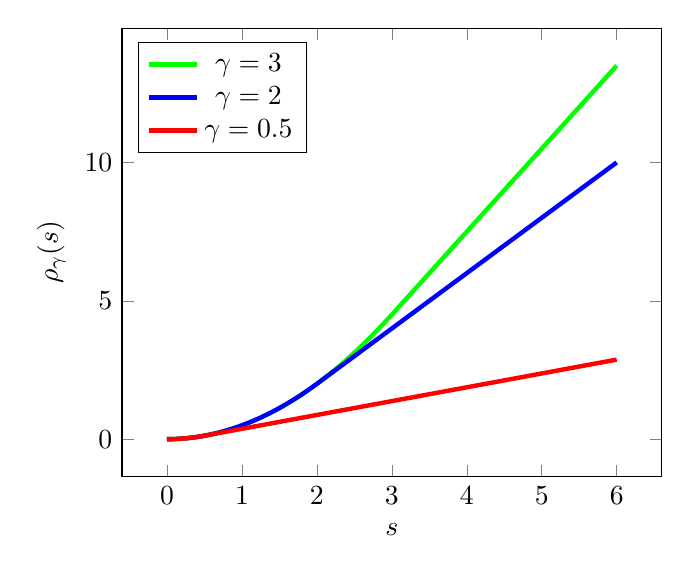
\begin{tikzpicture}
			\begin{axis}[
			xlabel=$s$,
			ylabel={$\rho_\gamma(s)$},
			legend pos=north west
			]
			% p_2(x)
			\addplot[green, ultra thick, domain=0:3]{0.5*x^2};
			\addlegendentry{$\gamma=3$}
			\addplot[blue, ultra thick, domain=0:2]{0.5*x^2};
			\addlegendentry{$\gamma=2$}
			\addplot[red, ultra thick, domain=0:0.5]{0.5*x^2};
			\addlegendentry{$\gamma=0.5$}
			
			\addplot[green, ultra thick, domain=3:6]{3*abs(x)-0.5*(3)^2};
			
			\addplot[blue, ultra thick, domain=2:6]{2*abs(x)-0.5*(2)^2};
			
			\addplot[red, ultra thick, domain=0.5:6]{0.5*abs(x)-0.5*(0.5)^2};
			
			\end{axis}
			\end{tikzpicture}
		}
	\end{center}
\end{frame}

\begin{frame}[t]{The $\epsilon$-insensitive Huber Function $g_\gamma^\epsilon(t)$}
	\begin{center}
		
		$f^{\epsilon}_\gamma(\mathbf{e}) = \underset{i \in [m]}{\sum} g^{\epsilon}_\gamma(\bar{\mathbf{e}}_i)$ with: \\
		
		$g^{\epsilon}_\gamma(t) = \left\{\begin{array}{lcc} 0 & si & \vert t \vert \leq \epsilon\\\rho_\gamma(\vert t \vert - \epsilon)   & si & \vert t \vert \geq \epsilon\\
		\end{array}
		\right.$
	\end{center}
	
\end{frame}

\section{The study case}

\begin{frame}[t]{Study case}
	
	\[(R(\lambda,k))\;\;\underset{\beta,\mathbf{e},\mathbf{z}}{min}\;\;f^\epsilon_\gamma (\mathbf{e}) + \lambda {\parallel \beta \parallel}_1\;\;s.t.\;\;(1)\]
	\[\mathbf{y} - X \beta = \mathbf{e}\;\;(2)\]
	\[\mbox{If}\;\;\mathbf{z}_j = 1\;\;\mbox{then}\;\;\beta_j = 0\;\;\forall j \in [n]\;\;(3)\]
	\[Co(\mathbf{z})\leq k\;\;(4)\]
	\[\underset{j \in J1_i}{\sum} \mathbf{z}_j \leq 1\;\;\forall i \in [n_1]\;\;(5)\]
	\[\underset{j \in J2_i}{\sum} \mathbf{z}_j = 1\;\;\forall i \in [n_2]\;\;(6)\]
	\[\mathbf{z}_{j_1} = \mathbf{z}_{j_2}\;\;\forall j_1,j_2 \in B_i\;\;\forall i \in [n_B]\;\;(7)\]
	\[\beta_j \geq 0\;\;\forall j \in J^+,\;\;\beta_j \leq 0\;\;\forall j \in J^-\;\;(8)\]

\end{frame}

\begin{frame}[t]{Study case (II)}
	
	\[(R(\lambda,k))\;\;\underset{\beta,\mathbf{e},\mathbf{z}}{min}\;\;f^\epsilon_\gamma (\mathbf{e}) + \lambda {\parallel \beta \parallel}_1\;\;s.t.\;\;(1)\]
	\[ \cdots \]
	\[\mathbf{z}_{j_1} + \mathbf{z}_{j_2} \leq 1\;\;\forall (j_1,j_2) \in Jc\;\;(9)\]
\[\beta \in \mathbb{R}^n,\;\;\mathbf{e} \in \mathbb{R}^m,\;\;\mathbf{z} \in {\lbrace 0,1 \rbrace}^n\;\;(10)\]

	
\end{frame}

\section{Roadmap}


\begin{frame}[t]{Road}
\textbf{Objective:} Find a set of solutions with values close to the optimal, this is {\it a path of Approximate Solutions} 

\begin{enumerate}
	\item Formulation of $ R(\lambda, k)$.
	\item Obtaining valid values for BigM values. 
		BigMs too big $\implies$ numerical problems, inefficiency of algorithms. 
		BigMs too small $ ~ implies $ good solutions removed. 
		\item {\it Local Holistic Searches}: Distances, Neighborhoods and Complexity function are presented on $\mathbf{z}$, which we will call Holistic, that adapt naturally to the case study, to obtain solutions locally optimal.
		\item Algorithms for the construction of the Approximate Solutions 	Path combining (2.) and (3.)
\end{enumerate}
\end{frame}



\end{document}
